\section{Theory}
	\subsection{Four Probe Method}
		The Four-Probe method is a widely used technique in materials science and condensed matter physics for accurate measurement of resistivity in materials. It is preferred over the conventional Two-Probe method due to its inherent advantages in minimizing errors caused by contact resistance. Four equally spaced collinear probes are used to make electrical contact with the surface of the material, with separate pairs of terminals to carry current and sense voltage. This configuration allows for precise voltage and current measurements, independent of the contact resistance, leading to more accurate and reliable resistivity measurements.

		To set up a Four-Probe measurement, the probes are carefully positioned on the sample surface, to form a known probe spacing. A known current is passed through the outer probes, and the voltage drop across the inner probes is measured as shown in \hyperref[th:1]{Figure 1}. The resistivity of the material can then be calculated using the measured voltage and current values, along with the probe spacing and geometry, following established mathematical formulas, such as the Van der Pauw method.
		
		The Four-Probe method offers several advantages over the Two-Probe method. Firstly, it eliminates errors associated with contact resistance, which can be a significant source of inaccuracy in resistivity measurements. Secondly, it allows for precise and simultaneous voltage and current measurements, leading to improved accuracy and reproducibility. Additionally, the Four-Probe method can be used to measure resistivity in a wide range of materials, including thin films, bulk samples, and even highly resistive materials. Overall, the Four-Probe method is a reliable and widely used technique for accurate resistivity measurements in materials research and characterization.
		
		\begin{figure}[h]
			\centering
			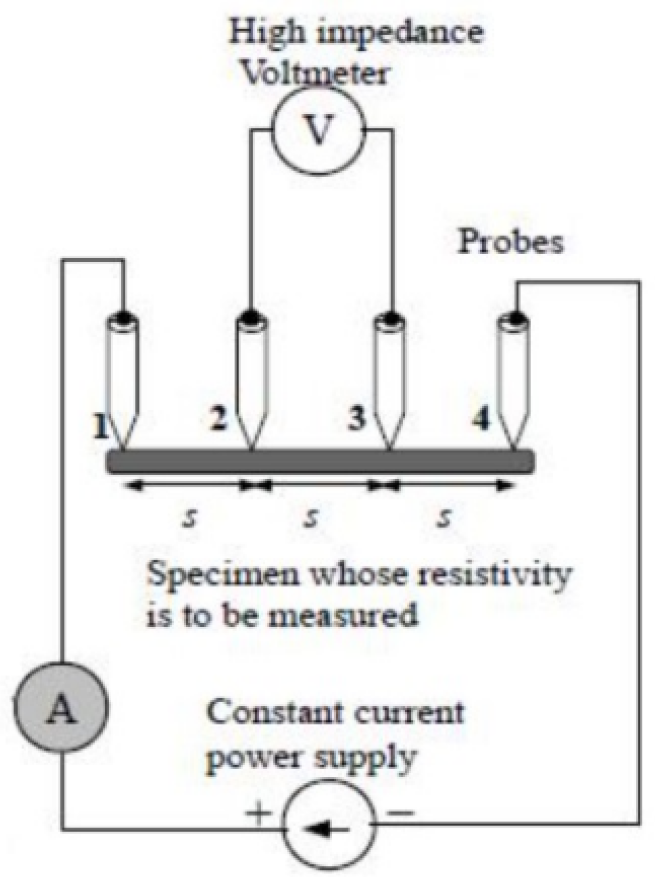
\includegraphics[width=0.5\columnwidth]{images/th1.png}
			\caption{Four-Probe method setup for resistivity measurement}
			\label{th:1}
		\end{figure}

	\subsection{For semi-infinite conducting material}
		A hemispherical equipotential surface develops at a probe when current flowing from a semi-infinite material is dispersed isotropically. The potential drop at an inner probe when two probes of different distances and opposing polarity are considered is:

		$$V = \frac{\rho_0I}{2\pi}\left(\frac{1}{r_1}-\frac{1}{r_2}\right)$$

		where $\rho_0$ is the resistivity, I is the current passed through the outer electrode and $r_1$ and $r_2$ is the distance from the probe $1$ and probe $4$ respectively. The floating potential across the inner terminals is determined by the following equation when evenly spaced probes are taken into account.

		$$V=\frac{\rho_0I}{2\pi S}$$

		S is the probe spacing. The resistivity of the material can be calculated using the following equation:

		\begin{equation}
			\rho_0 = \frac{V}{I} 2\pi S
			\label{eq:1}
		\end{equation}

	\subsection{For thin sheet placed on a non-conducting surface}
		Since the thickness of the samples are small compared to the probe distance, a correction factor for it has to be applied. If the bottom surface is not conducting, then the corrected formula for resistivity will be:

		$$\rho = \frac{\rho_0}{G_7(\sfrac{W}{S})}$$

		where W is the width of the sample and $G_7(\sfrac{W}{S})$ is the required correction factor defined as follows:

		$$G_7(\sfrac{W}{S}) = 1 + 4 \frac{S}{W}\sum_{n=1}^{\infty} f(S,\;W,\;n) $$

		$$f(S,\;W,\;n) = \left[\frac{1}{\sqrt{\left(\frac{S}{W}\right)^2+n^2}} - \frac{1}{\sqrt{\left(\frac{2S}{W}\right)^2+4n^2}}\right]$$

		For smaller values of $\frac{W}{S} (\le 0.25)$, we can approximate the value of $G_7(\sfrac{W}{S})$ as:

		$$G_7(\sfrac{W}{S}) = \frac{2S}{W}\ln(2)$$

		From these equations we get:

		\begin{equation}
			\rho = \frac{\pi}{\ln(2)}W\frac{V}{I}
			\label{eq:2}
		\end{equation}

	\subsection{Relation of resistivity the band gap of a
	semiconductor}

		If $E_g$ is the band gap energy, $k_B = 8.6\times 10^{-5} eV/K$ is the Boltzmann constant, and $T$ is the temperature in Kelvin:

		\begin{equation}
			E_g = 2k_B\frac{\ln(\rho)}{\sfrac{1}{T}}
			\label{eq:3}
		\end{equation}

		where $\frac{\ln(\rho)}{\sfrac{1}{T}}$ can be determined from the slope of as appropriate $\ln(\rho)$ vs. $\sfrac{1}{T}$ plot.